%
%  愛知工業大学 情報科学部 情報科学科
%    要旨集用LaTeXテンプレート(2016.11.28)
%
%  original by Nobuhiro Ito
%  revised by Susumu Suzuki & Masashi Morimoto on 2016.11.28
%
\documentclass{jarticle}
\pagestyle{empty}

%% レイアウト
\setlength{\topmargin}{-10.4mm}
\setlength{\headheight}{0mm}
\setlength{\headsep}{0mm}
\setlength{\textheight}{262mm}
\setlength{\textwidth}{180mm}
%\setlength{\topskip}{7mm}
\setlength{\evensidemargin}{-10.4mm}
\setlength{\oddsidemargin}{-10.4mm}
\setlength{\columnsep}{8mm}

%% パッケージ環境
% graphicx: 画像読み込み
%  dvipdfmxをドライバ指定することでpdf/png/jpeg形式の図を利用可能
%  異なるドライバを利用する場合はそのドライバ指定に変更
% \usepackage{graphicx} % suzuki
\usepackage[dvipdfmx]{graphicx} % suzuki
% subcaption: subfigureを置き換えたパッケージ(複数の図用)
% \setlength{\footskip}{12mm}
% \usepackage{subfigure}	 % suzuki
\usepackage{subcaption} % suzuki
% color:文章に色をつけたいとき
%  利用例:\textcolor{red}{文章}
% \usepackage{color}
\usepackage{booktabs}
\usepackage{setspace}
\usepackage{url}
\urlstyle{sf}

% 行間調整
\setstretch{0.9}

%sectionのフォントサイズ修正
\makeatletter
\def\section{\@startsection {section}{1}{\z@}{2.5ex plus -1ex minus -.2ex}{1.3 ex plus .1ex}{\large\bf}}
\makeatother

%subsectionのフォントサイズ修正
\makeatletter
\def\subsection{\@startsection {subsection}{1}{\z@}{1.5ex plus -1ex minus -.4ex}{0.3 ex plus .1ex}{\bf}}
\makeatother

\begin{document}
\twocolumn[

\begin{center}
%タイトル
{\LARGE \textbf{声に対する印象を用いた\\合成音声ライブラリ探索システムに関する研究}}\\
%サブタイトル
%{\Large \textbf{必要に応じてサブタイトル}}
\end{center}

\begin{center}
% 著者
\begin{tabular}{cccc}
% 1名の場合
\multicolumn{4}{c}{K21066 清水洸世}\\
% 2名の場合
%& K11002 愛工七音 & X11003 愛工頼音 &\\
% 3名の場合
%K11001 愛工総和 & K11002 愛工今鹿 & X11003 愛工姫星&\\
% 4名の場合
% K11001 愛工総和 & K11002 愛工今鹿 & X11003 愛工姫星& X11004 愛工緑輝\\
% 指導教員
\multicolumn{4}{c}{\textbf{指導教員} 梶克彦}
\end{tabular}
\hspace{2zw}
\end{center}
]

%--------------------------------------------
\section{はじめに}
\label{sec:intro}
人の歌声や喋り声を人工的に再現する音声合成ソフトとそのライブラリは非常に数多く存在しているが,それらを十分な数聞き込み目的に合った声を探し当てることは困難である.
その問題に対し,声に対する印象を数値で表現する研究\cite{impression}や,数値化した印象を利用し合成音声ライブラリの探索を行う研究\cite{dnn}は存在するが,ユーザが実際に利用できるようなサービスとしての提供を目的とはしたものは未だ無い.

本研究では,ライブラリの声に対する印象を数値化し,ユーザの求める声に近いライブラリを探索できるWebサービスを提案する.
探索対象は,特に利用できるライブラリが特に多く,後述する声質に関するアンケートが既存するUTAU音源ライブラリとした.
ユーザが手軽に利用できるような実装や,印象の数値化を機械学習を用いて自動化することでサービス上にないライブラリをユーザが追加できるなどUGCとしての機能の提供を目指す.

\begin{figure}[h]
  \centering
  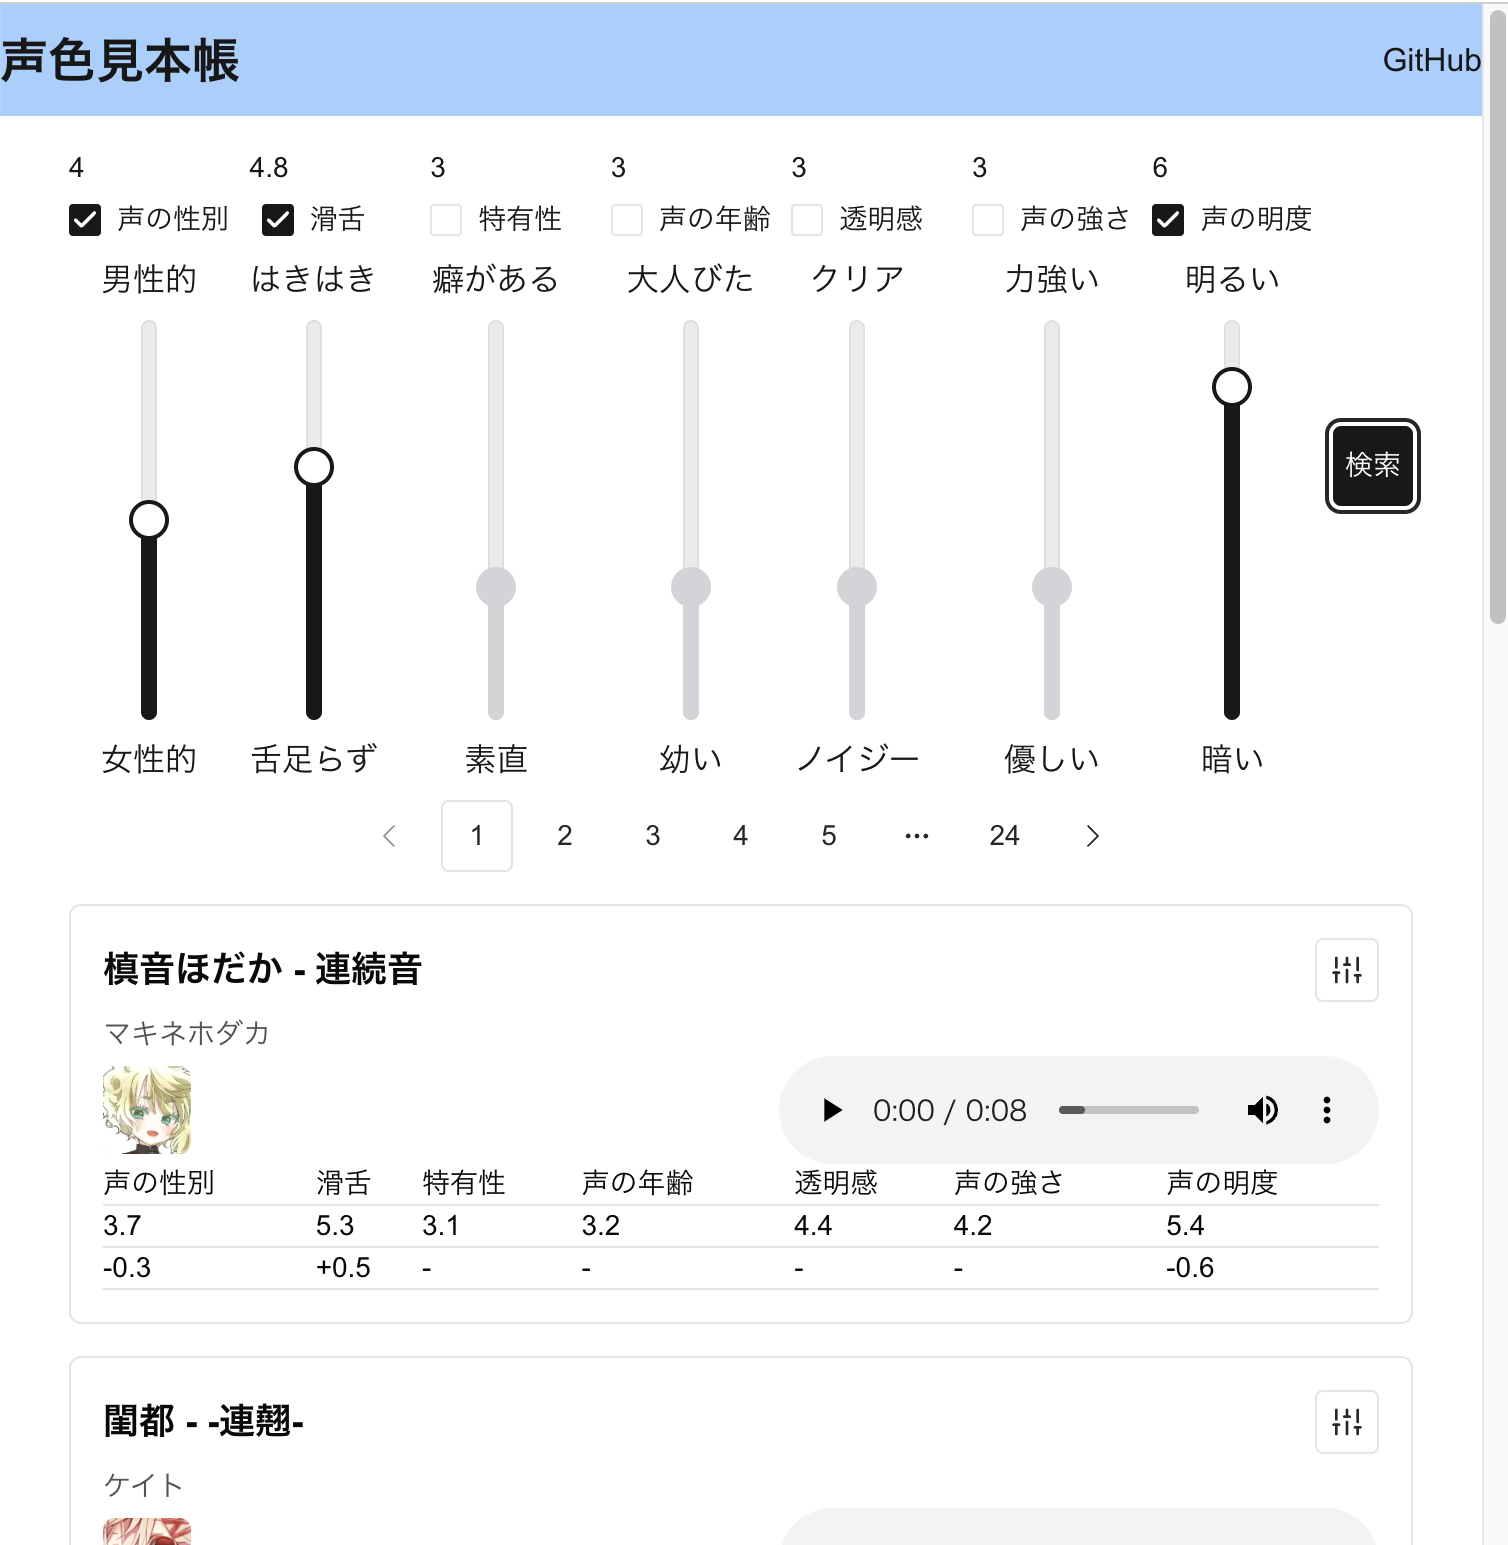
\includegraphics[width=0.9\linewidth]{fig/site_image.png}
  \caption{作成したサービス「声色見本帳」の画面}
  \label{fig:site_image}
\end{figure}

%--------------------------------------------
\section{評価スコアを推定するモデルの構築}
本研究ではまずUTAU音源ライブラリに対して声質に対する評価スコアを付与するため,ライブラリの音響特徴量から評価スコアを推定する機械学習モデルを作成する.
音響特徴量として,ライブラリの音声からMFCC,ZCR,F1〜F4の周波数を抽出する.
評価スコアの教師データには,既存のUTAU音源声質アンケートを用い,推定する評価の軸も同アンケートに基づく7軸を用いる.

本研究で利用するUTAU音源声質アンケートはニコニコ大百科上で提言されたUTAU音源ライブラリに対する声の特徴を評価するためのアンケート規格\cite{utausurvey}であり,現在までにこの規格を用いて250種以上のUTAU音源ライブラリに対してアンケートが行われている.
このアンケートは表\ref{tab:survey}に示す7項目について,それぞれ1から7までの7段階評価で10件以上のアンケート調査を行い,その平均を評価値としている.

\begin{table}[htb]
    \centering
    \caption{UTAU音源声質アンケートの評価軸}
    \label{tab:survey}
    \begin{tabular}{c|cc}
        \hline
        評価軸 & 低い値の示す表現語 & 高い値の示す表現語 \\
        \hline
        声の性別 & 女性的 & 男性的 \\
        滑舌 & 舌足らず & はきはき \\
        特有性 & 素直 & 癖がある \\
        声の年齢 & 幼い & 大人びた \\
        透明感 & ノイジー & クリア \\
        声の強さ & 優しい & 力強い \\
        声の明度 & 暗い & 明るい \\
        \hline
    \end{tabular}
  \end{table}

\subsection{モデルの構築}
本研究では,音響特徴量から評価スコアを推定するモデルとしてAdaBoost Regressorを採用した.
この選択は,評価スコアと音響特徴量がともに連続値であること,また予備実験において離散モデルでの学習時に過学習の傾向が見られたことに基づいている.

教師データには,アンケート結果をまとめた配布ファイルに記載されているライブラリの中から,学習に利用できる条件の整った168ライブラリを使用した.
データセットは学習データとテストデータに分割し,ランダムに選択した30\%をテストデータ,残りの70\%を学習データとして使用した.

モデルの構築にはPythonライブラリPyCaretを使用し,7つの評価軸それぞれについて独立したモデルを作成した.
各モデルは,先述の音響特徴量を入力として受け取り,対応する評価軸のスコアを出力として推定する.

\subsection{モデルの評価} \label{sec:eval}
構築したモデルによる推論の精度を評価するため,テストデータに対する予測スコアと実際のスコアの相関係数を求め,その結果を表\ref{tab:score_coor}に示した.
図\ref{tab:score_coor}では,横軸は評価軸を,縦軸はテストデータにおける実際の値と推測された値との相関係数を示している.
その結果,最も低い「声の年齢」は0.20とかなり低いものの,残りの6軸では0.49から0.66程度,そのうち最も高い「声の強さ」では0.66と,ある程度の相関が見られた.

\begin{figure}[h]
    \centering
    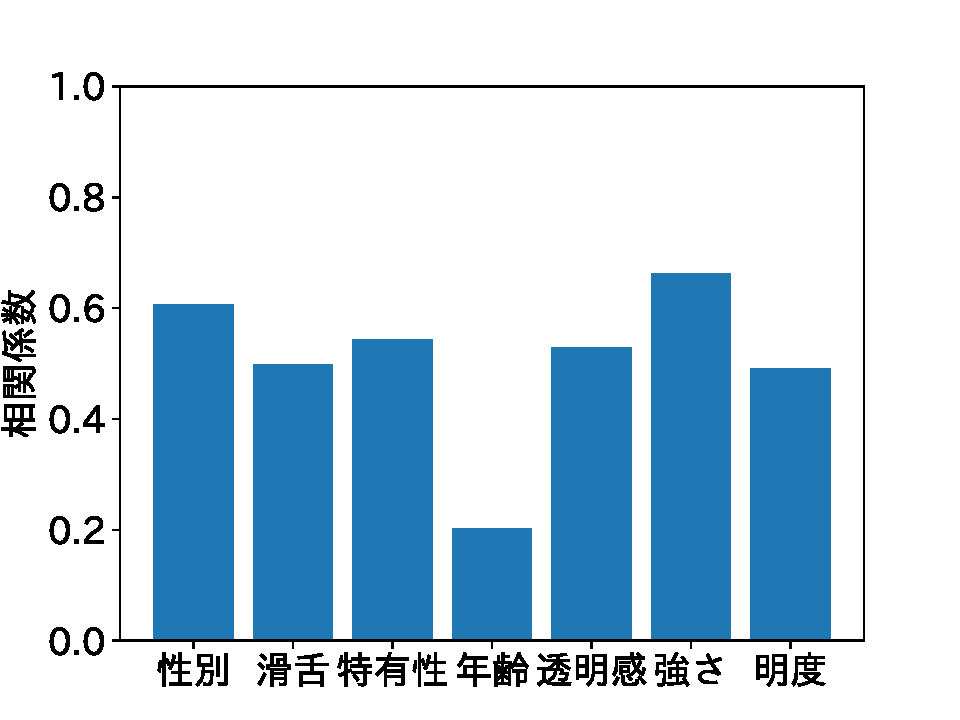
\includegraphics[width=\linewidth]{fig/model_quality_coor.pdf}
    \caption{テストデータとの相関係数}
    \label{tab:score_coor}
\end{figure}

相関係数が最も高かった「声の強さ」と最も低かった「声の年齢」について,実際の値と予測値の散布図を図\ref{fig:scatter}に示す.
散布図から,「声の強さ」では対角線上に沿った分布が見られるのに対し,「声の年齢」では予測値が中央値付近(3〜5)に集中し,実際の値との相関が低いことが確認できる.
この予測値の中央集中傾向は,「声の性別」と「声の強さ」を除く他の評価軸においても同様に観察できる.
この傾向は現在使用している音響特徴量が声質の印象を十分に表現できていないことが原因の一つであると考えられ,今後の改善が課題である.

\begin{figure}[h]
  \centering
  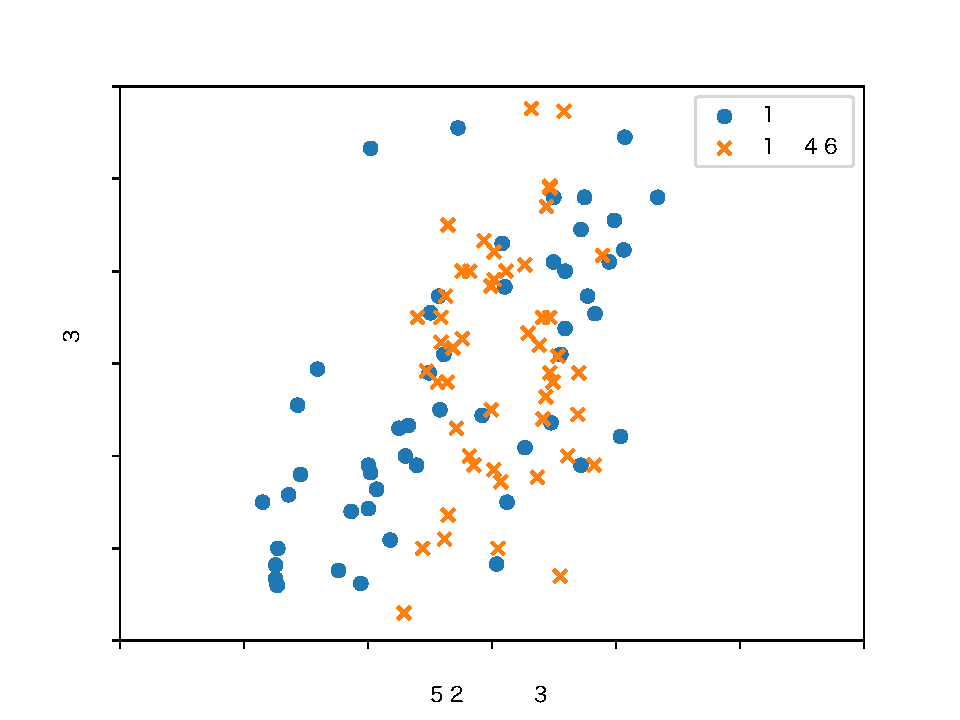
\includegraphics[width=\linewidth]{fig/scatter.pdf}
  \caption{実際の値と推測された値の散布図}
  \label{fig:scatter}
\end{figure}


%--------------------------------------------
\section{声色見本帳}
本研究で提案するサービス「声色見本帳」は,ユーザが求める声の評価スコアを入力し,その評価スコアに近い合成音声ライブラリを探索・提案するサービスである.
ユーザは大量に存在する合成音声ライブラリの中から,自身が用途に合わせて求める声に近いライブラリを手軽に探すことができる.
サービスはWebサービスとして実装し,ユーザはブラウザ上で利用できる.

\subsection{要求仕様}
本研究で提案するサービスについての要求仕様を以下に示す.
ユーザは求める声の評価スコアを入力し,その評価スコアに近いUTAU音源ライブラリを探索できる.
探索結果画面からはライブラリのサンプルボイスを再生したり,配布ページへのリンクを確認できる.
本サービスは探索のみを目的とし,ライブラリを直接ダウンロードできる機能は提供しない.
また,ユーザが新しいライブラリを追加できる機能も提供する.
この機能によって,新たに公開されたライブラリや,サービスに登録されていないライブラリに対しても将来的に探索が可能となる.

\subsection{実装}
探索機能では,ユーザは各評価軸に対してスライダーを用いて1〜7の評価スコアを入力できる.
重視しない評価軸はチェックボックスで無効化でき,選択された軸のみで平方ユークリッド距離による類似度計算を行う.
計算結果に基づき,求める声質に近いライブラリから順に表示する.

ライブラリ詳細表示機能では,ライブラリとバージョン名,評価スコア,サンプル音声,アイコン,配布URLなどの情報を提供する.
サンプル音声は「かえるのうた」をPythonライブラリ「ScoreDraft」で事前に合成したものを使用する.

ライブラリ追加機能では,ユーザは未登録のライブラリをzipファイルでアップロードすることで,自動的に音響特徴量を抽出し,構築済みの機械学習モデルで評価スコアを推定する.
アップロード時には合わせて配布ページへのURLやライブラリの名前などのメタデータの入力を要求する.
推定結果とメタデータ,合成したサンプルボイスをデータベースに登録することで,新規ライブラリも探索対象として利用でき,サービスの即時性と持続可能性を高めることができる.

%--------------------------------------------
\section{今後の課題}
まずは\ref{sec:eval}節でも述べたように機械学習モデルの改善が挙げられる.
具体的には,音響特徴量を追加することで声質の印象をより正確に表現できるようにすることが考えられる.
現状では母音の音響特徴量のみを使用しているが,子音にまつわるものや音素間の時間的な遷移を表現できる特徴量の追加などが考えられる.
またサービスとしての利便性向上も課題として挙げられ,探索時の類似度指標の改善や,ライブラリ情報の更新・修正・削除機能の実装などの改善を行うことでより利便性の高いサービスを目指したい.

%--------------------------------------------
\begin{thebibliography}{9}

\bibitem{impression}
金礪 愛,中野 倫靖,後藤 真孝,菊池 英明,
歌声の印象評価尺度の構築に基づく多様な印象の自動推定手法.
情報処理学会論文誌,Vol.57,No.5,pp.1375-1388,2016

\bibitem{dnn}
横森文哉,大柴まりや,森勢将雅,小澤賢司,
スペクトル包絡情報を入力としたDeep Neural Networkに基づく歌声のための声質評価
情報処理学会音楽情報科学研究会,Vol.2015-MUS-107,No.61,1-6,2015

\bibitem{utausurvey}
ニコニコ大百科,
UTAU音源声質アンケートとは,
\url{https://dic.nicovideo.jp/a/utau音源声質アンケート}

\end{thebibliography}
\end{document}

%%% Local Variables:
%%% mode: japanese-latex
%%% TeX-master: t
%%% End:
